\documentclass{article}

% if you need to pass options to natbib, use, e.g.:
%     \PassOptionsToPackage{numbers, compress}{natbib}
% before loading neurips_2019

% ready for submission
\usepackage{neurips_2019}
\usepackage[pdftex]{graphicx}
% to compile a preprint version, e.g., for submission to arXiv, add add the
% [preprint] option:
%     \usepackage[preprint]{neurips_2019}

% to compile a camera-ready version, add the [final] option, e.g.:
     %\usepackage[final]{neurips_2019}

% to avoid loading the natbib package, add option nonatbib:
%     \usepackage[nonatbib]{neurips_2019}

\usepackage[utf8]{inputenc} % allow utf-8 input
\usepackage[T1]{fontenc}    % use 8-bit T1 fonts
\usepackage{hyperref}       % hyperlinks
\usepackage{url}            % simple URL typesetting
\usepackage{booktabs}       % professional-quality tables
\usepackage{amsfonts}       % blackboard math symbols
\usepackage{nicefrac}       % compact symbols for 1/2, etc.
\usepackage{microtype}      % microtypography

\title{Investigating Network Architectures on Canonical 1D Partial Differential Equations}

% The \author macro works with any number of authors. There are two commands
% used to separate the names and addresses of multiple authors: \And and \AND.
%
% Using \And between authors leaves it to LaTeX to determine where to break the
% lines. Using \AND forces a line break at that point. So, if LaTeX puts 3 of 4
% authors names on the first line, and the last on the second line, try using
% \AND instead of \And before the third author name.

\author{%
  Alejandro Francisco Queiruga\thanks{} \\
  Energy Geosciences Division\\
  Lawrence Berkeley National Lab\\
  Berkeley, CA 94609\\
  \texttt{afqueiruga@lbl.gov} \\
}

\begin{document}

\maketitle

\begin{abstract}
  This work performs a thorough empirical analysis of the application
  of neural networks to solving well understood partial differential
  equations. Only one spatial dimension is treated to , where pentiful analytical solutions can be evaluated to machine precision to provide datasets with no artifacts.
  Burger's equation and the Korteweg-de Vries equation are treated,
  which even are challenging to solve numerically due
  to their nonlinearity and exhibition of shock fronts even in one spatial dimension.
\end{abstract}

\section{Introduction}

Hypotheses:
\begin{enumerate}
  \item Adding adverserial training will improve stability
  \item need 2 history for wave equation
  \item AE will be bad
    \item need a unet or FC to do heat eq
\end{enumerate}

Most extremely challanging physical systems are extremely challenging to describe due to unknown underlying physics or intractable complexities with traditional approaches. Analysis of dynamics data through neural networks and deep learning is a hot topic and very promising approach to learn predictive tools, but the properties are not yet well understood. The problem of discovering dynamics can be stated as follows:
\begin{equation}
\textrm{Given data }\, u_i^k=u(x_i,t_k), \,\textrm{find }f\textrm{ such that }\, u^{k+1}=f(u^k)
\end{equation}
This paper seeks to explore the use of neural networks as an $f$ to discover predictive functions on well known equations (for which decent $f$s are already known.)\footnote{This approach is looking for a function that inputs an image returns and image. Another approach is to look for conditional scalar functions with coordinates as inputs, $u^{k+1}(x,y)=f(x,y|u^{k})$; this was not considered. }
Basic one dimensional partial differential equations are always useful to benchmark to any new numerical technique due to well understood properties and known analytical solutions, which can provide as much data as needed without artifacts from synthesis or acquisition.
Multiple standard types of architectures are applied to each of these
canonical equations.
The experiments are designed to take a few minutes of compute time training to replicate with datasets that even fit within a modern cache.
Applying intuition from well understood physics-and-math-up approaches will improve future approaches, providing insights that can hopefully be applied to problems without known physical descriptions but similarities to canonical problems.


Neural networks have rightfully been given a lot of attention to apply to many domains.
The structure of many physical sciences problems is similar to image and speech processing: e.g., PDEs are just grid or graph convolutions once discretized.
Applying generative adverserial networks to perform forecasting and super resolutions

Koopman theory and dynamic mode decomposition are traditional approaches to discovering dynamics.
Instead of searching for nonlinear transforms to find linear operators, but how well can we seek nonlinear operators?
As opposed to fiting to known PDE terms, can we discover neural networks that match known approximations to the operators?  Can neural networks offer us a richer space to find nonlinear operators?

However, how much of this is due to inherent biases? 
Problems in the physical sciences require more than fuzzy-qualities such as probabilistic classification or pretty behavior in the ``eyeball norm'': fine-grained properties such as regression accuracy and numerical stability are important.
It has even been suggested that the structure of CNNs and not the learning stage is the dominating factor to their performance [deep image prior,\cite{ulyanov_deep_2018,zador_critique_2019}. Thus, devising architectures specifically for physical applications 


Multiple equations are known to not fit into a PDE context. E.g., burger's equation becomes discontinuous, and ANOTHER EQUATION NEEDS FRACTIONAL DERIVATIVES. The scale of known PDEs may even be intractable in certain contexts, such as attempting to apply Navier-Stokes to the global climate.


A variety of rich datasets are available for this task, such as the John Hopkins Turbulence dataset. However, it is wise to give attention to problems with known solutions when crafting new methods. Towards this end, this work focuses on verifying methods 1D PDEs, providing small datasets.



Of further interest, how do we predict very far out in the future? If it is possible to learn a model that predicts $t+\Delta t$, how do we predict far in the future given only one initial datapoint? Feeding a model's input into itself is natural---$u^{k+n}=f(f(...f(u^k)$---but this requires stability on $f$.

From the history numerical methods, the well known and understood finite difference method solve the problem using stencils:
\begin{equation}
  u^{k+1}_{i} = u^k_{i}+\mathtt{stencil}\left( u^k_{i-1}, u^k_{i},u^{k}_{i+1}; \Delta x, \Delta t\right)
\end{equation}
This architecture corresponds to a fringe case neural network: a 3-weight 1D convolutional neural network (CNN) with no bias and no activation function. 
The classical stencil for the heat equation is $u_{xx}\approx\frac{\Delta t}{\Delta x^2} \left(1 u_{i-1} - 2 u_{i} +1 u_{i+1}\right)$.
Verifying that these coefficients can be derived by the optimization algorithm is a good first step: below, it is shown that the standard ADAM optimizer will discover this stencil, albeit slowly.
These architectures are called ``PureStencil'' and ``PureLinear''.

The equations used in the investigation are summarized in Table \ref{tab:pdes}. (Technically, all but one are actually 2D when including time.)
These include the linear Poisson's equation, an elliptic equation; the heat equation, a parabolic equation; and the wave Equation, a hyperbolic equation: all three have well-understood finite difference stencils. 
Burgers' equation, a conservative nonlinear equation known for
  producing sharp fronts,
The Korteweg-de Vries Equation equation, a conservative nonlinear equation known for
producing sharp fronts,
(One could argue that the notion of a PDE even breaks down for Burgers' equation due to the existence of discontinuities: how can finite differences even be applied?)

\begin{table}
  \caption{\label{tab:pdes}PDEs under investigation}
  \begin{tabular}{lll}
    \hline
    Name & Equation & Properties\\
    \hline\hline
    Poisson Equation & $u_{xx} = f $ & Linear, elliptic, static \\\hline\
    Heat Equation & $u_{t} = k u_{xx} $ & Linear, parabolic \\\hline
    Wave Equation & $u_{tt} = c^2 u_{xx} $ & Linear, hyperbolic\\\hline
    Advection Equation & $u_{t} + a u_x = 0 $ & Linear, hyperbolic\\\hline
    Burgers' Equation & $u_{t} + u_x u = 0 $ & Nonlinear, shock waves \\\hline
    Viscous Burgers' Equation & $u_{t} + u_x u = \nu u_{xx} $ & Nonlinear, general analytical solution \\\hline
    Korteweg-de Vries Equation & $\partial_t u + 6 u \partial_x u + \partial_{xxx}u = 0$ & Shallow Waves \\\hline
  \end{tabular}
\end{table}

A dataset is created for each equation where 10 trajectories are solved analytically and evaluated on a grid of 41 points in x and 100 snapshots in $t$. The analytical solutions and their implementations can be found in the accompanying source code. Six trajectories are used for training, two are used for testing, and two are used for validation by self-iterating on the initial snapshot. 


\section{Models}

\subsection{Architectures}
\begin{figure}
  \centering
  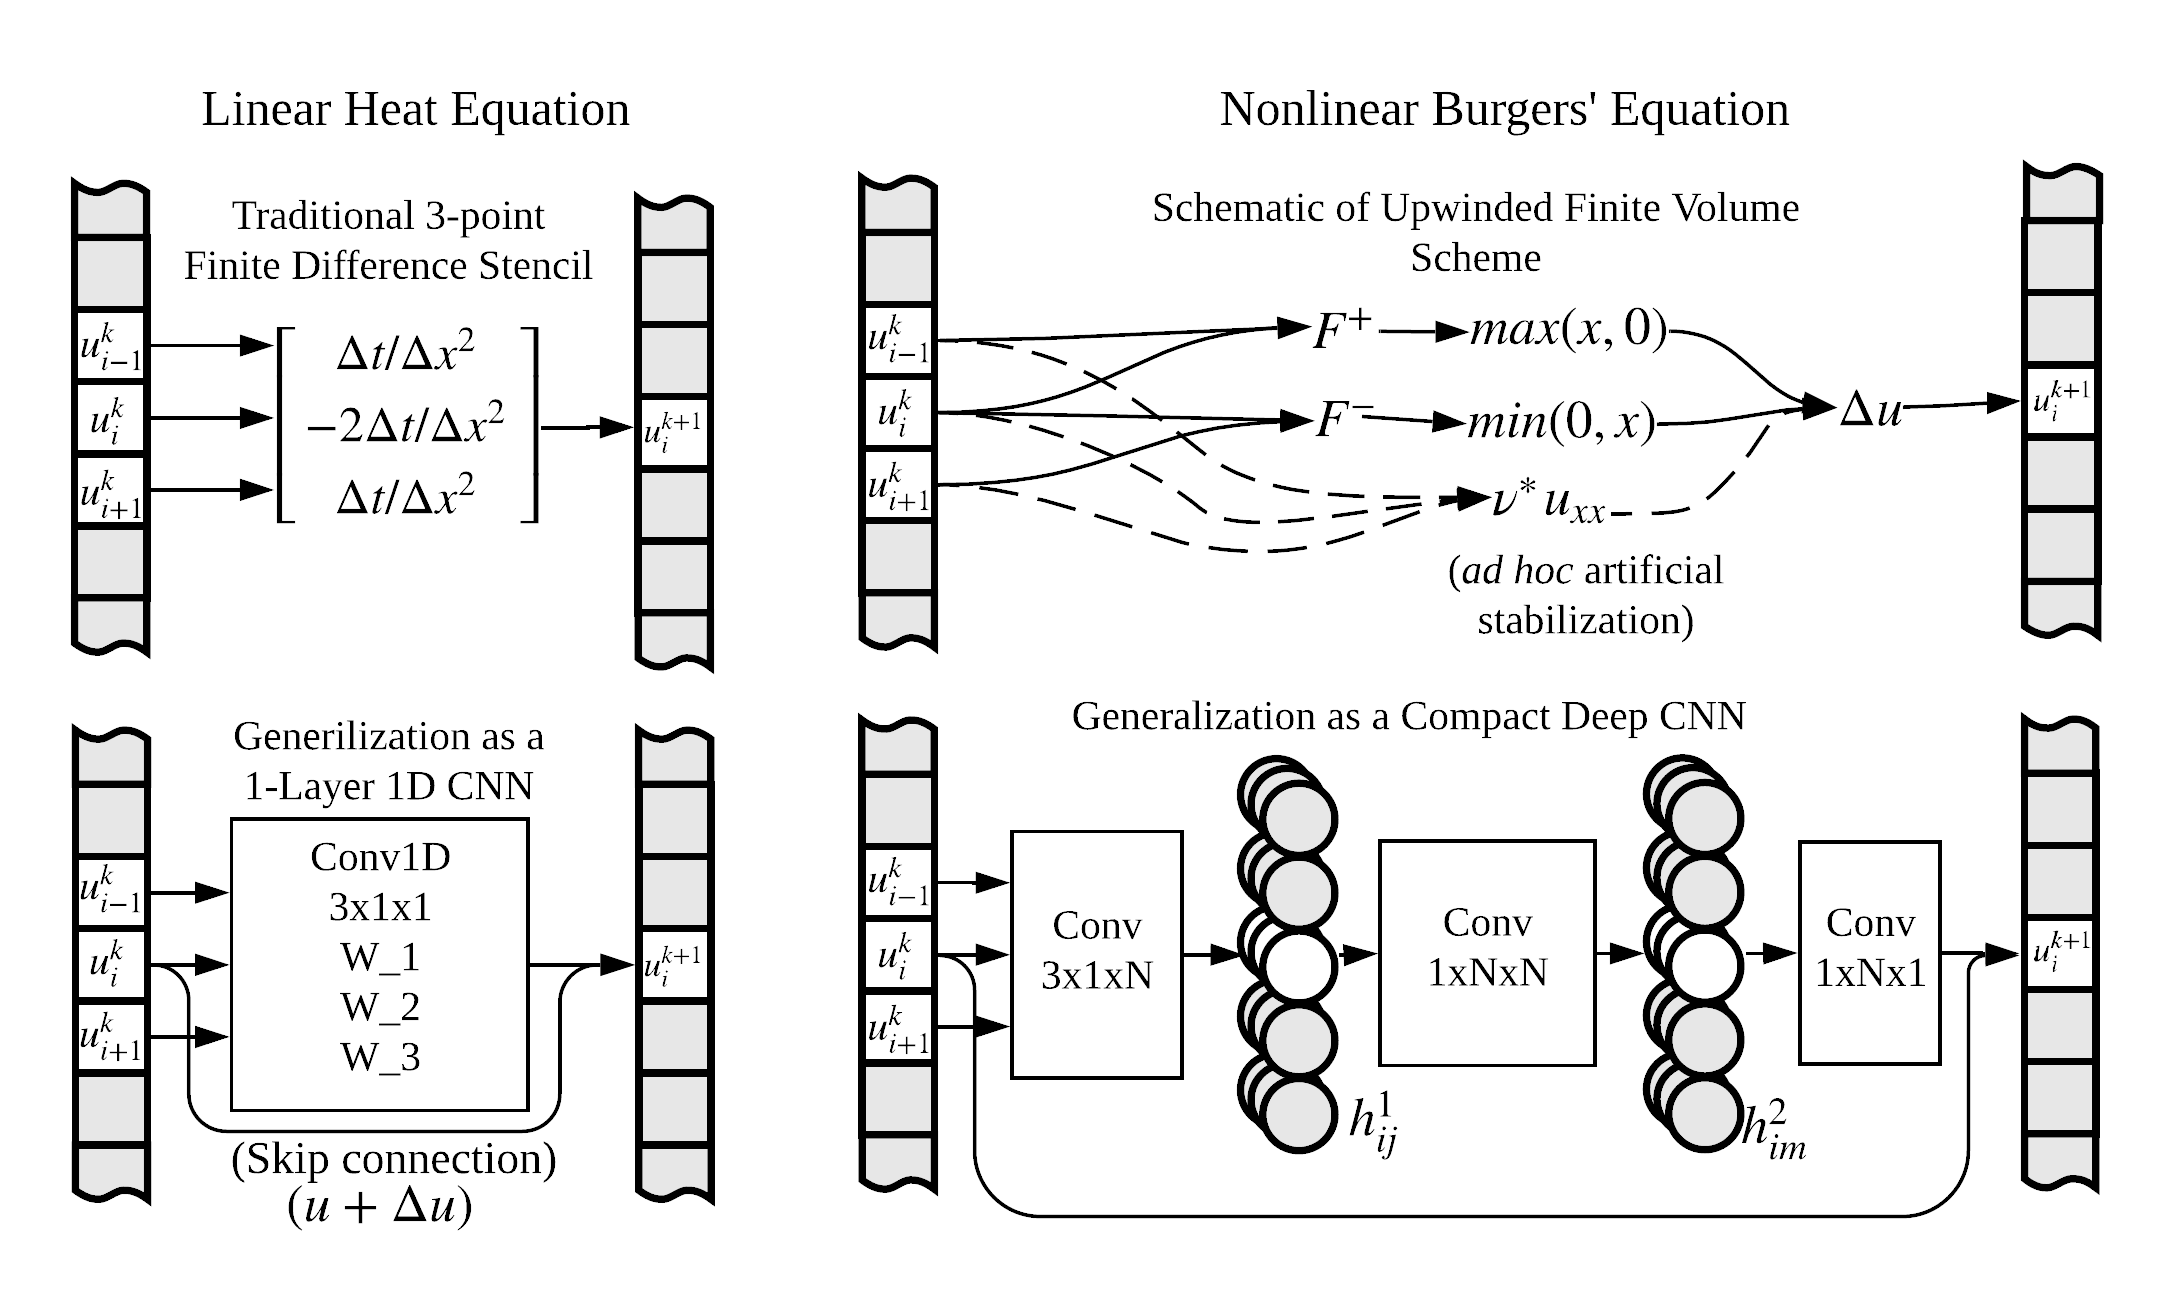
\includegraphics[width=5in]{CNN_FDM.png}  
  \caption{Diagrams of the networks.}
\end{figure}


The modle input is an $N_x$ array. Boundary conditions are neglected for this investigation. When
performing recurrent prediction, the values at the edges of the domain are set to
the known analytical solution to ensure that improper treatment of the
boundaries do not contaminate the results, yielding pure Dirrichlet
boundary conditions every. The boundary domain is extended to the
sencil width. The model output is thus padded by the correct amount of 0s to make the output an $N_x$ array.


\begin{table}
  \caption{\label{tab:network}Network Architectures Used}
  \begin{tabular}{llc}
    \toprule
    Name & Description & No. of Parameters \\
    \midrule
    PureStencil & Conv(3,1,bias=False) & 3 \\
    PureLinear & Linear($N_x$,$N_x-2$,bias=False) & 1,599 \\
    FCMLP & & \\
    Linear Conv & & 3 \\
    Pure-ConvMLP & &  \\
    Autoencoder & & \\
    U-Net & &  \\
    Recurrent & & \\
    \midrule
    Discriminator & Conv(3,1),Pool(3,1), AdptPool(1), Sigmoid & \\
    \bottomrule
  \end{tabular}
\end{table}

Question: Do we want to learn $u^{k+1}$ or $\Delta u^{k+1}$?
The paper THAT ONE ABOUT RESNET showed a technique to describe residual networks as iterative time stepping methods to improve training. The effect on training is tried by adding a skip connection to all of the models--- $f(x)=\mathbf{net}(x)+x$---so that $\mathbf{net}$ learns the rate. This would further allow changing $\Delta t$ or generalize to other time integration schemes, but this was not explored.

\subsection{Loss functions}
The time frequency of snapshots used for training will affect training.
Recall the Courant–Friedrichs–Lewy (CFL) condition dictating the ratio
of spatial and temporal discretization spacings to ensure stability
for explicit schemes: $\delta t / \delta x < C$ or $\delta t / \delta
x^2<C$ for some positive $C$.

The standard metric is the L2 loss function:
\begin{equation}
L\left(u^k,u^{k+1}\right) = \left\| u^{k+1}_i-f(u^k) \right\|_2^2.
\end{equation}
The cost function to minimize at each step is $N_{batch}^{-1}\sum_{x,y\in batch} L(y,x)$.

Multiple input steps effects the network architecture:
\begin{equation}
L\left(\left\{u^k,u^{k-1}...u^{k-P}\right\},u^{k+1}\right) = \left| u^{k+1}_i-f(u^k,...u^{k-P}) \right|
\end{equation}

It is desired to obtain a model that can operate on its own outputs, so that behavior can be included in training:
\begin{eqnarray}
L_n\left(u^k,\left\{u^{k+1},u^{k+2}...\right\}\right) =  \left| u^{k+1}-f(u^k) \right| + \lambda_1  \left| u^{k+2}-f \circ f(u^k) \right| \nonumber \\+ \lambda_2  \left| u^{k+3}-f \circ f \circ f(u^k) \right| + ...
\end{eqnarray}
where $\lambda_i$ are weighting coefficients. 

Adverserial training is also considered. A conditional discriminator $D(y|x)$ is optimized which learns, given $x$, determine if $y$ is the datum or the model prediction. For these problems, no stochastic effects are included, and the model and evaluation of the discrimanor are perfectly deterministic. Thus, the inclusion of adverserial is essentially {\em learning a loss function}, replacing the mean-squared-error loss with potentially something better:
\begin{equation}
L_D(y,x)= \left(1 - D\left(f(x)|x\right) + D\left(y|x\right)\right)/2
\end{equation}
\footnote{Averaging this loss function over a batch the same way as the others yields the $\mathbb{E}_x[1-D(f(x))]-\mathbb{E}_y[D(y)]$ equation of traditional GANs, but using ``expected value'' does not quite apply to a fully deterministic model.}

\section{Implementation Details}

The datasets were created using Sympy and are 1.6MB in total. The entire study is implemented in PyTorch. The experiments were designed to run in a few minutes each using a GPU instance on Google Colaboratory. The source code and datasets can be found at https://github.com/{\em hidden for blind review.}


\section{Heat Equation}

The first sanity check was to derive the $[1,-2,1]$ stencil from the heat equation dataset with a three-parameter CNN.
Testing the algorithms ADAM, Rprop, and SGD on learning rates of $0.1, 10^{-2}, 10^{-3}, 10^{-4}$, and $10^{-5}$, only ADAM converged to the right answer with $0.1$ and $10^{-2}$. Increasing from single precision to double precision did not change this result. Single precision with a learning rate of $0.1$ was used for the rest of the studies.
This test also verified that the dataset met the CFL condition by assigning the ``PureStencil'' CNN parameters to the expected answer, enabling the testing of this barrier.

\begin{figure}
  \centering
  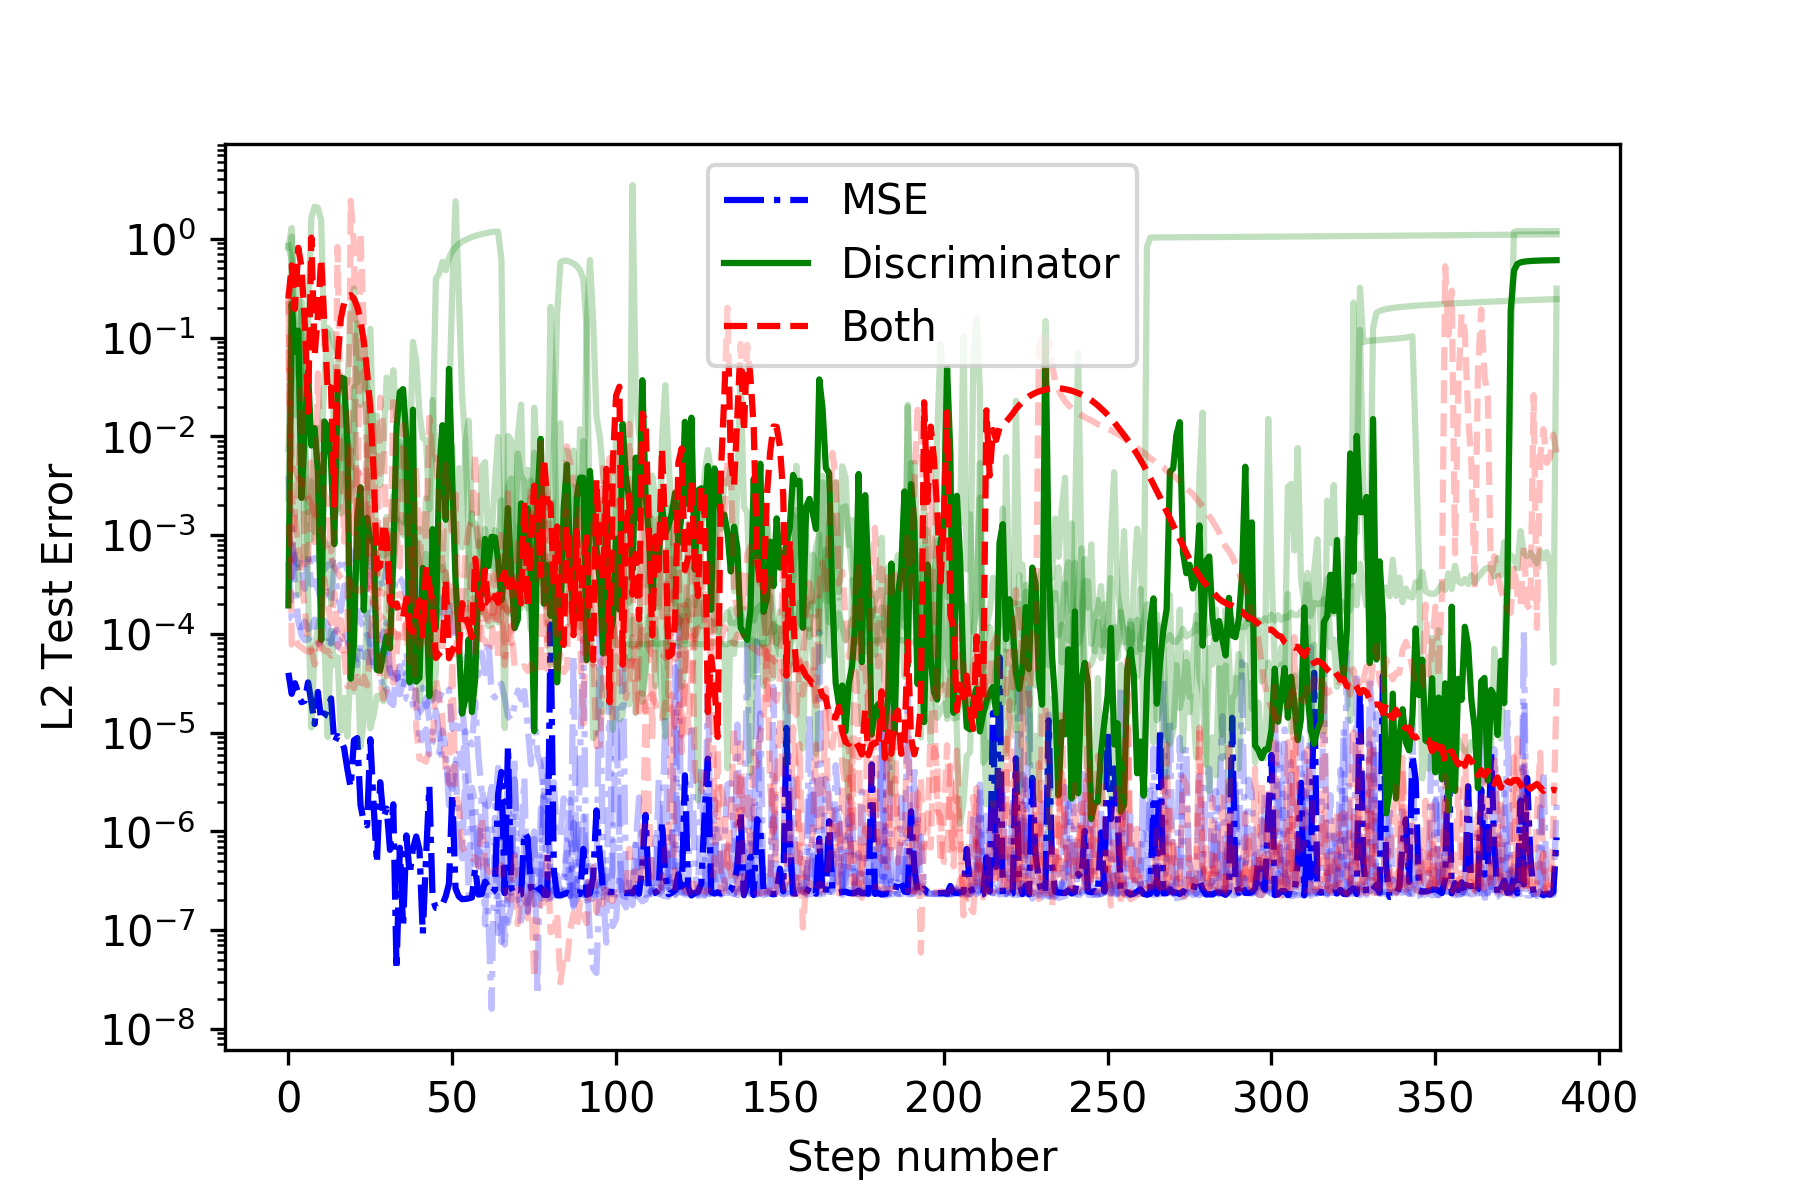
\includegraphics[width=5in]{3pt_L2_loss.png}
  \caption{Convergence of 3-parameter CNN to the expected stencil
    using L2 optimization and adversarial
    training. $10^{-7}$ error is possibly the best in single precision.}
\end{figure}

\begin{table}
  \caption{The convolutional weights learning by the 3 training
    methods for five randomly initialized runs. The weights are
    divided by $k \Delta t / \Delta x^2$ to normalize to $1,-2,1$.}
  \begin{tabular}{rrr|rrr|rrr}
    \hline
    &MSE& & &Adversary& & &Both& \\
\hline
 0.997 & -1.995 & 0.997 & 1.398 & -1.149 & 1.401 & 1.073 & -2.149 & 1.077 \\
 0.997 & -1.995 & 0.998 & 1.058 & -3.196 & 0.956 & 0.994 & -2.000 & 0.995 \\
 0.998 & -1.996 & 0.998 & 1.512 & -0.824 & 1.624 & 0.595 & -1.502 & 0.732 \\
 0.998 & -1.994 & 0.999 & 1.084 & -1.154 & 1.116 & 1.000 & -2.001 & 1.000 \\
 0.998 & -1.995 & 0.998 & 1.392 & -0.558 & 1.394 & 1.000 & -1.999 & 1.000 \\
\hline
\end{tabular}
  \end{table}

Purely adverserial training with a learned discriminator does not learn the same stencil. It appears that the discriminator only learns the ``parabolic'' shape to it, but not the magnitude. Combining the discriminator loss and L2 loss improve training and converges to the correct stencil with correct magnitude. The L2 testing loss of both is shown in Figure \ref{fig:l2adverse}.
%When observing the learned values during training, it was observed that the $[1,-2,1]$ ``shape'' of the stencil was trained quickly, but that it took a longer time to optimize to the magnitude.
These results suggest caution to using a purely GAN-type training for physics problems where accuracy is important. The ability to detect the shape of the operator is promising; the {\em author(s)} hypothesize that the discriminator may help with issues such as stability in more complex systems.

\section{Conclusion}
\label{sec:conclusion}

We show that a fringe case of CNN architecture corresponds to a standard finite difference stencil, and converges to the expected coefficients using popular optimizers for NNs on both L2 loss and a learned loss function through adversial training.
Deep CNNs were successfully derived for solving Burgers' equation accurately {\em and } stably.



This analogy allows us to interpret the output of our learning algorithms, and guide the design of new architectures for these problems.
This work hopes to provide a simple, well understood benchmark for proving recently demonstrated ML methods for solving physical systems developing ML methods for solving physical systems (and remaining as a tiny unit test to the codebases!)
By finding this area of overlap between solving PDEs and deep learning, we can seek to bridge the gap and transfer knowledge between the two fields. For example, can methods for L-stable implicit high-order ODE integration be applied to transformer networks?



% \subsection{Margins in \LaTeX{}}

% Most of the margin problems come from figures positioned by hand using
% \verb+\special+ or other commands. We suggest using the command
% \verb+\includegraphics+ from the \verb+graphicx+ package. Always specify the
% figure width as a multiple of the line width as in the example below:
% \begin{verbatim}
%    \usepackage[pdftex]{graphicx} ...
%    \includegraphics[width=0.8\linewidth]{myfile.pdf}
% \end{verbatim}
% See Section 4.4 in the graphics bundle documentation
% (\url{http://mirrors.ctan.org/macros/latex/required/graphics/grfguide.pdf})

% A number of width problems arise when \LaTeX{} cannot properly hyphenate a
% line. Please give LaTeX hyphenation hints using the \verb+\-+ command when
% necessary.

\subsubsection*{Acknowledgments}

{\em left out for blind review}
% Use unnumbered third level headings for the acknowledgments. All acknowledgments
% go at the end of the paper. Do not include acknowledgments in the anonymized
% submission, only in the final paper.

% \section*{References}

% \medskip

% \small

\bibliographystyle{plainnat}
\bibliography{zotero}

\end{document}
